\section{Minimization by the Simplex Method}
In this section, you will learn to solve linear programming minimization problems using the simplex method.
\begin{enumerate}
    \item Identify and set up a linear program in standard minimization form.
    \item Formulate a dual problem in standard maximization form.
    \item Use the simplex method to solve the dual maximization problem.
    \item Identify the optimal solution to the original minimization problem from the optimal simplex tableau.
\end{enumerate}

In this section, we will solve the standard linear programming minimization problems using the simplex method. Once again, we remind the reader that in the standard minimization problems all constraints are of the form $ax + by \geq c$.

The procedure to solve these problems was developed by Dr. John Von Neuman. It involves solving an associated problem called the dual problem. To every minimization problem there corresponds a dual problem. The solution of the dual problem is used to find the solution of the original problem. The dual problem is a maximization problem, which we learned to solve in the last section. We first solve the dual problem by the simplex method.

From the final simplex tableau, we then extract the solution to the original minimization problem. Before we go any further, however, we first learn to convert a minimization problem into its corresponding maximization problem called its dual.

\begin{example}\label{example_convert_minimization_into_dual}
    Convert the following minimization problem into its dual.

    Minimize
    \[ Z = 12x_1 + 16x_2 \]
    Subject to:
    \begin{align*}
        x_1 + 2x_2        & \geq 40    \\
        x_1 + x_2         & \geq 30    \\
        x_1 \geq 0; \quad & x_2 \geq 0
    \end{align*}
\end{example}

\begin{solution}
    To achieve our goal, we first express our problem as the following matrix.
    \[
        \begin{array}{cc|c}
            1  & 2  & 40 \\
            1  & 1  & 30 \\
            \hline
            12 & 16 & 0  \\
        \end{array}
    \]
    Observe that this table looks like an initial simplex tableau without the slack variables. Next, we write a matrix whose columns are the rows of this matrix, and the rows are the columns. Such a matrix is called a transpose of the original matrix. We get:
    \[
        \begin{array}{cc|c}
            1  & 1  & 12 \\
            2  & 1  & 16 \\
            \hline
            40 & 30 & 0  \\
        \end{array}
    \]

    The following maximization problem associated with the above matrix is called its dual.

    Maximize
    \[ Z = 40y_1 + 30y_2 \]
    Subject to:
    \begin{align*}
        y_1 + y_2         & \leq 12    \\
        2y_1 + y_2        & \leq 16    \\
        y_1 \geq 0; \quad & y_2 \geq 0
    \end{align*}

    Note that we have chosen the variables as \( y \)'s, instead of \( x \)'s, to distinguish the two problems.
\end{solution}

\begin{example}\label{example_min_max_dual_graphically}
    Solve both the minimization problem and its dual maximization problem graphically.
\end{example}

\begin{solution}
    Our minimization problem is as follows.

    Minimize
    \[ Z = 12x_1 + 16x_2 \]
    Subject to:
    \begin{align*}
        x_1 + 2x_2        & \geq 40    \\
        x_1 + x_2         & \geq 30    \\
        x_1 \geq 0; \quad & x_2 \geq 0
    \end{align*}

    We now graph the inequalities:
    \begin{center}
        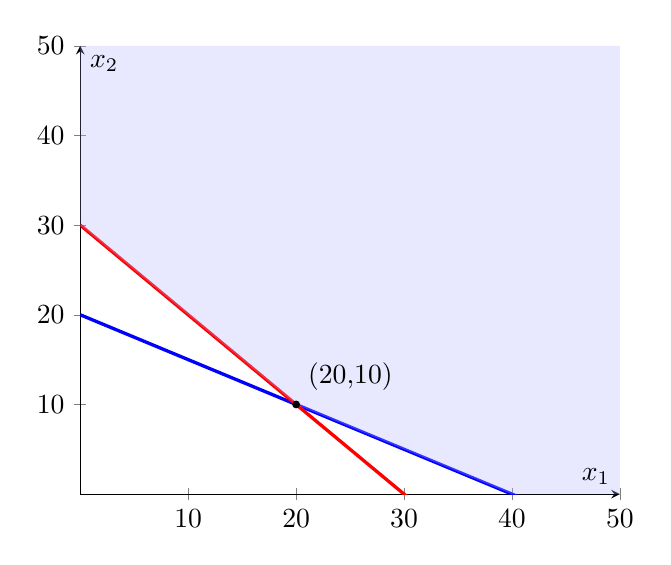
\begin{tikzpicture}
            \begin{axis}[
                    xmin=0, xmax=50,
                    ymin=0, ymax=50,
                    axis lines=middle,
                    xlabel=$x_1$,
                    ylabel=$x_2$,
                    % grid=major,
                    % grid style=dashed,
                ]

                % x1 + 2x2 >= 40
                \addplot[domain=0:50, samples=200, color=blue, very thick]{(40 - x)/2} node[pos=1, anchor=south west] {$x_1 + 2x_2 = 40$};

                % x1 + x2 >= 30
                \addplot[domain=0:50, samples=200, color=red, very thick]{30 - x} node[pos=1, anchor=south west] {$x_1 + x_2 = 30$};

                % Feasibility region
                \fill[blue!30, opacity=0.3] (axis cs:20,10) -- (axis cs:40,0) -- (axis cs:50,0) -- (axis cs:50,50) -- (axis cs:0,50)-- (axis cs:0,30) -- cycle;

                % Corner points
                \node[label={60:{(20,10)}},circle,fill,inner sep=1pt] at (axis cs:20,10) {};
                % \node[label={180:{(30,0)}},circle,fill,inner sep=2pt] at (axis cs:30,0) {};

            \end{axis}
        \end{tikzpicture}
    \end{center}

    We have plotted the graph, shaded the feasibility region, and labeled the corner points. The corner point (20, 10) gives the lowest value for the objective function and that value is 400.

    Now its dual is:
    Maximize
    \[ Z = 40y_1 + 30y_2 \]
    Subject to:
    \begin{align*}
        y_1 + y_2         & \leq 12    \\
        2y_1 + y_2        & \leq 16    \\
        y_1 \geq 0; \quad & y_2 \geq 0
    \end{align*}

    We graph the inequalities:
    \begin{center}
        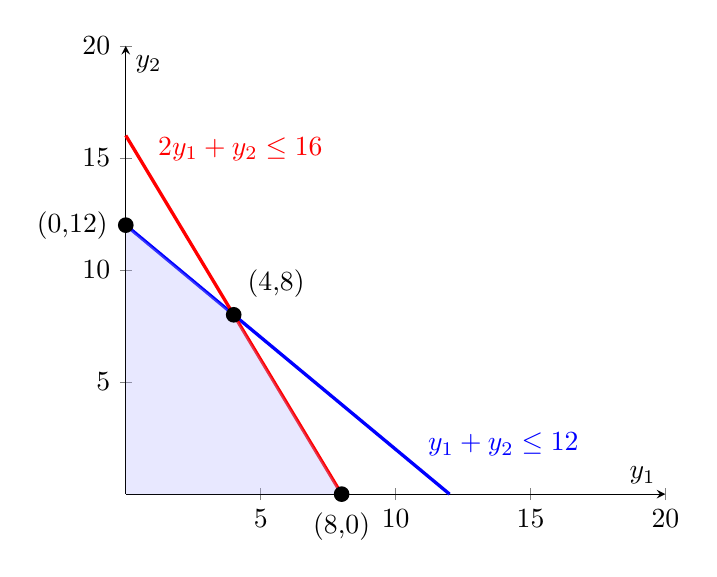
\begin{tikzpicture}
            \begin{axis}[
                    xmin=0, xmax=20,
                    ymin=0, ymax=20,
                    axis lines=middle,
                    xlabel=$y_1$,
                    ylabel=$y_2$,
                    clip = false,
                    % grid=major,
                    % grid style=dashed,
                ]

                % y1 + y2 <= 12
                \addplot[domain=0:12, samples=200, color=blue, very thick]{12 - x} node[pos=.9, anchor=south west] {$y_1 + y_2 \leq 12$};

                % 2y1 + y2 <= 16
                \addplot[domain=0:8, samples=200, color=red, very thick]{16 - 2*x} node[pos=.1, anchor=south west] {$2y_1 + y_2 \leq 16$};

                % Feasibility region
                \fill[blue!30, opacity=0.3] (axis cs:0,0) -- (axis cs:0,12) -- (axis cs:4,8) -- (axis cs:8,0) -- cycle;

                % Corner points
                \node[label={180:{(0,12)}},circle,fill,inner sep=2pt] at (axis cs:0,12) {};
                \node[label={60:{(4,8)}},circle,fill,inner sep=2pt] at (axis cs:4,8) {};
                \node[label={270:{(8,0)}},circle,fill,inner sep=2pt] at (axis cs:8,0) {};

            \end{axis}
        \end{tikzpicture}
    \end{center}

    Again, we have plotted the graph, shaded the feasibility region, and labeled the corner points. The corner point (4, 8) gives the highest value for the objective function, with a value of 400.
\end{solution}

The reader may recognize that Example \ref{example_min_max_dual_graphically} above is the same as Example \ref{niki_geometry} in section \ref{section_maximization_geometry}. It is also the same problem as Example \ref{niki_simplex} in section \ref{section_maximization_simplex}, where we solved it by the simplex method.

We observe that the minimum value of the minimization problem is the same as the maximum value of the maximization problem; in Example \ref{example_min_max_dual_graphically} the minimum and maximum are both 400. This is not a coincidence. We state the duality principle.

\begin{definition}
    \textbf{The Duality Principle}
    The objective function of the minimization problem reaches its minimum if and only if the objective function of its dual reaches its maximum.  And when they do, they are equal.
\end{definition}

Our next goal is to extract the solution for our minimization problem in Example \ref{example_convert_minimization_into_dual} from the corresponding dual. To do this, we solve the dual by the simplex method.

\begin{example}
    Find the solution to the minimization problem in Example \ref{example_convert_minimization_into_dual} by solving its dual using the simplex method. We rewrite our problem:
    Minimize
    \[ Z = 12x_1 + 16x_2 \]
    Subject to:
    \begin{align*}
        x_1 + 2x_2        & \geq 40    \\
        x_1 + x_2         & \geq 30    \\
        x_1 \geq 0; \quad & x_2 \geq 0
    \end{align*}
\end{example}

\begin{solution}
    The dual is:
    Maximize
    \[ Z = 40y_1 + 30y_2 \]
    Subject to:
    \begin{align*}
        y_1 + y_2         & \leq 12    \\
        2y_1 + y_2        & \leq 16    \\
        y_1 \geq 0; \quad & y_2 \geq 0
    \end{align*}

    Recall that we solved the above problem by the simplex method in Example \ref{niki_simplex}, section \ref{section_maximization_simplex}. Therefore, we only show the initial and final simplex tableau.

    The initial simplex tableau is:
    \[
        \begin{array}{c c c c c | c c}

            y_1 & y_2 & x_1 & x_2 & Z & C  &     \\

            1   & 1   & 1   & 0   & 0 & 12 & y_1 \\
            2   & 1   & 0   & 1   & 0 & 16 & y_2 \\
            \hline
            -40 & -30 & 0   & 0   & 1 & 0  & Z   \\
        \end{array}
    \]

    Observe an important change. Here our main variables are \(y_1\) and \(y_2\) and the slack variables are \(x_1\) and \(x_2\).

    The final simplex tableau reads as follows:
    \[
        \begin{array}{ccccc|c}
            y_1 & y_2 & x_1 & x_2 & Z & C   \\
            0   & 1   & 2   & -1  & 0 & 8   \\
            1   & 0   & -1  & 1   & 0 & 4   \\
            \hline
            0   & 0   & 20  & 10  & 1 & 400 \\
        \end{array}
    \]

    A closer look at this table reveals that the \(x_1\) and \(x_2\) values along with the minimum value for the minimization problem can be obtained from the last row of the final tableau. We have highlighted these values by the arrows.

    \[
        \begin{array}{ccccc|c}
            y_1 & y_2 & x_1      & x_2      & Z & C        \\
            0   & 1   & 2        & -1       & 0 & 8        \\
            1   & 0   & -1       & 1        & 0 & 4        \\
            \hline
            0   & 0   & 20       & 10       & 1 & 400      \\
                &     & \uparrow & \uparrow &   & \uparrow \\
        \end{array}
    \]
\end{solution}

We restate the solution as follows:
The minimization problem has a minimum value of 400 at the corner point $(20, 10)$.

\begin{summarybox}{Minimization by the Simplex Method}
    \begin{enumerate}
        \item Set up the problem.
        \item Write a matrix whose rows represent each constraint with the objective function as its bottom row.
        \item Write the transpose of this matrix by interchanging the rows and columns.
        \item Now write the dual problem associated with the transpose.
        \item Solve the dual problem by the simplex method learned in section \ref{section_maximization_simplex}.
        \item The optimal solution is found in the bottom row of the final matrix in the columns corresponding to the slack variables, and the minimum value of the objective function is the same as the maximum value of the dual.
    \end{enumerate}
\end{summarybox}
